%% LyX 1.6.5 created this file.  For more info, see http://www.lyx.org/.
%% Do not edit unless you really know what you are doing.
\documentclass[oneside,english]{amsart}
\usepackage[T1]{fontenc}
\usepackage[latin9]{inputenc}
\usepackage[letterpaper]{geometry}
\geometry{verbose,tmargin=3cm,bmargin=3cm,lmargin=3cm,rmargin=3cm,headheight=3cm,headsep=3cm,footskip=3cm}
\usepackage{varioref}
\usepackage{amsthm}
\usepackage{graphicx}

\makeatletter
%%%%%%%%%%%%%%%%%%%%%%%%%%%%%% Textclass specific LaTeX commands.
\numberwithin{equation}{section}
\numberwithin{figure}{section}

\makeatother

\usepackage{babel}

\begin{document}

\title{Computational Physics: Assignment \#1}


\author{Micha Gorelick}

\maketitle

\section{Introduction}

The Lane-Emden equation,\[
\frac{d^{2}w(z)}{dz^{2}}+\frac{2}{z}\frac{dw(z)}{dz}+w(z)^{n}=0\]


describes the density profile of a star with polytropic index $n$.
This equation can be written as a system of two coupled ODE's,\begin{eqnarray*}
\frac{dw(z)}{dz} & = & v(z)\\
\frac{dv(z)}{dz} & = & -2\frac{v(z)}{z}-w(z)^{n}\end{eqnarray*}


and then solved using various Runge-Kutta methods. We will describe
our findings regarding numerical solutions of this equation using
forward Euler, RK2, RK4 and RK5.


\section{w profile}

Figure \vref{Flo:one} shows the results of solving Lane-Emden in
the case where $n=1$. This polytropic index is chosen because the
analytic solution is known and thus we can compute the L1 error of
the numerical solution. As such, we can get a sense of the convergence
rates of the schemes since, with dt as high as $\frac{10}{9}$, RK4
and RK5 still provide quite accurate results. Interestingly, we see
that RK5 does not greatly improve the results over RK4. This is a
direct result of the theorem by Butcher which states that RK schemes
greater than 4th order have lower order for systems of equations than
for single scalar problems%
\footnote{Given in class, Sept 16th, 2010%
}.

%
\begin{figure}
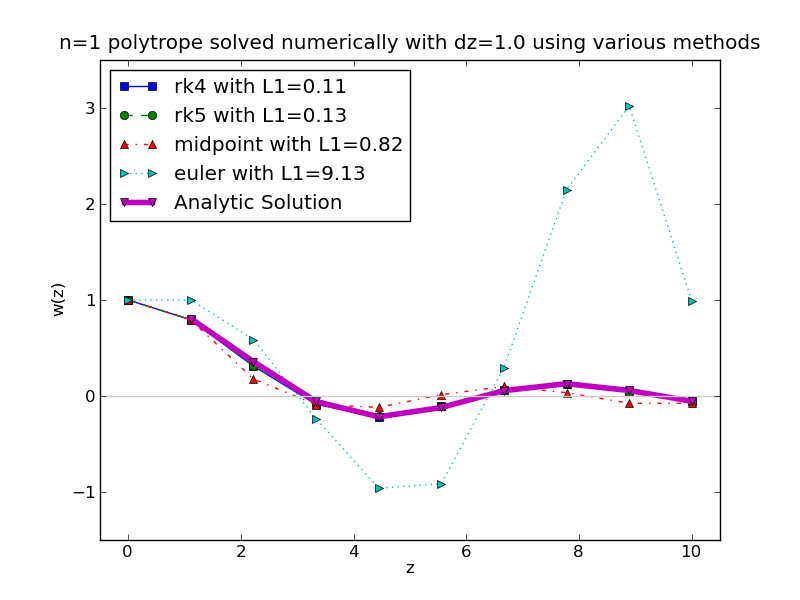
\includegraphics[width=1\textwidth]{images/one}\label{Flo:one}

\caption{Solutions for Lane-Emden with n=1, $z_{max}=10$ and $i_{max}=10$
for forward Euler, RK2, RK4 and RK5.}



\end{figure}



\section{Convergence Rate}

We can further analyze the properties of the various Runge-Kutta schemes
by calculating the convergence rates. Figure \vref{Flo:two} shows
how the L1 error scales with the chosen timestep. We can see that
Euler is first order, midpoint is second order, RK4 is fourth order
and finally that RK5 is effectively fourth order for this particular
system. This graph outlines how much better fourth order schemes are:
with every halving of the timestep, we get a quarter of the error!

%
\begin{figure}
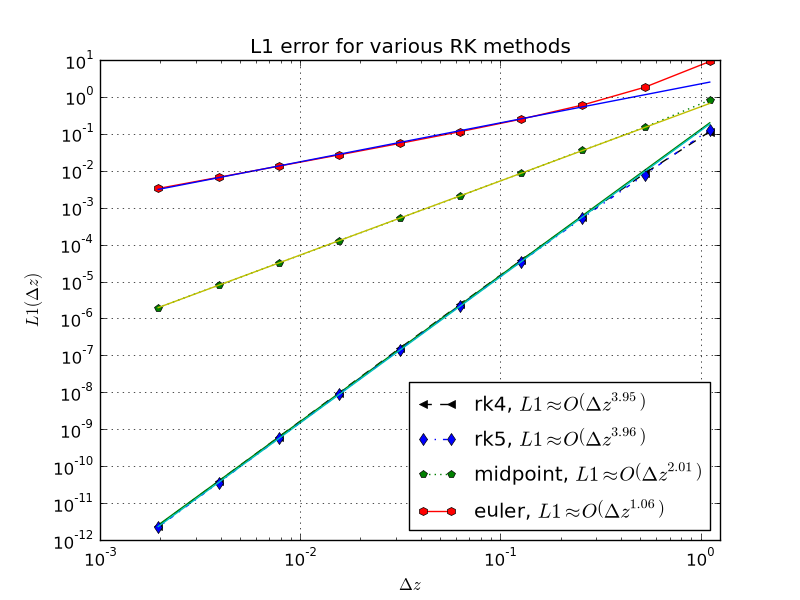
\includegraphics[width=1\textwidth]{images/two}\label{Flo:two}

\caption{Convergence rates for forward Euler, RK2, RK4 and RK5}

\end{figure}



\section{Finding the Radius of Stars}

Now that we have reliable numerical methods, we can solve for the
w-profile of non-analytic polytropic indices. Figure \vref{Flo:three}
shows the results of for the w-profile when $n\in{1,\frac{3}{2},3}$
which we use to find the radius of the star. 

For the previous solutions, we were not guaranteed to have integrated
to large enough z in order to see the root of $w(z)$. In order to
shed more light onto this issue, we have integrated all polyropes
with polytropic indices $n\in\{0,0.05,0.10,\cdots,4.95\}$ and founts
the roots. Then, we solve using least squares to find a relation for
the radius of the star given it's polytropic index. The solution is
shown in Figure \vref{Flo:four}. To further understand this, we first
realize that the polytropic index defined a relationship between the
pressure, $P$, and the density, $\rho$, of a system as $P\sim\rho^{1+\frac{1}{n}}$.
Since $\frac{1+n}{n}=\frac{c_{p}}{c_{v}}$ where $c_{p}$ is the specific
heat at constant pressure and $c_{v}$ is the specific heat at constant
volume, this can be seen as a change of the compressibility of the
gas for an adiabatic process.

%
\begin{figure}
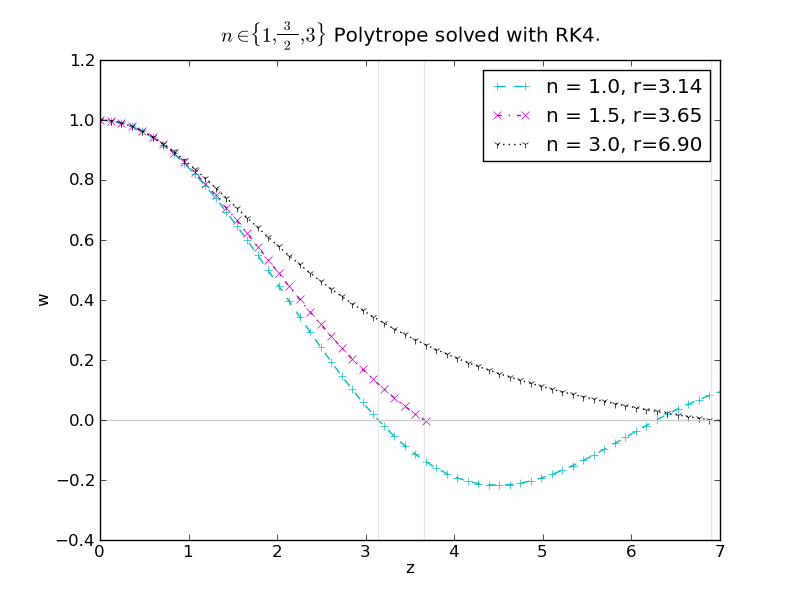
\includegraphics[width=1\textwidth]{images/three}\label{Flo:three}

\caption{Solutions for Lane-Emden with $n\in{1,\frac{3}{2},3}$ using RK4.}

\end{figure}


%
\begin{figure}
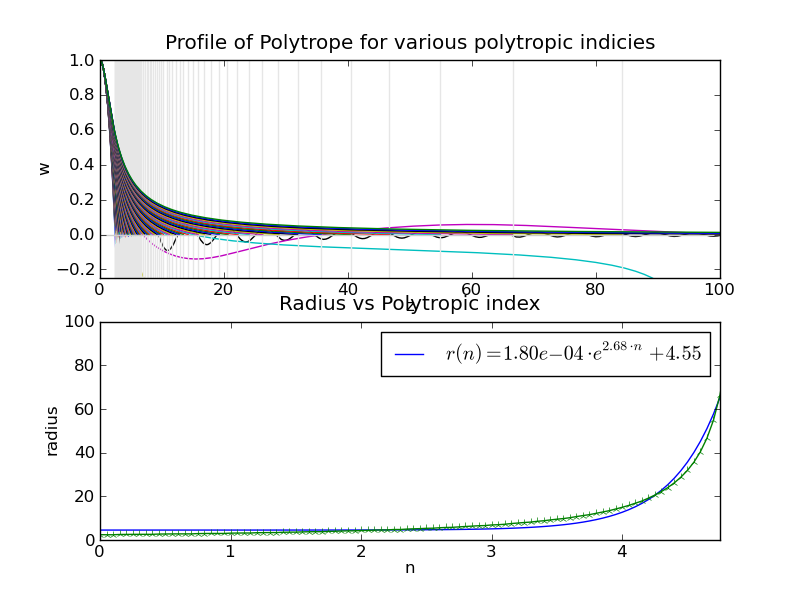
\includegraphics[width=1\textwidth]{images/four}\label{Flo:four}

\caption{Using RK4 and Least Squares to find a relation for $r(n)$.}

\end{figure}

\end{document}
